\chapter{Năng lượng, độ cong và bức xạ}

\lectureoverview{Mô hình Newton trở nên sáng tỏ hơn nhiều khi bỏ đi hai ràng buộc. Thứ nhất, một thiên hà đồng chuyển động không nhất thiết phải có tổng năng lượng đúng bằng 0; việc để năng lượng của nó là tùy ý đưa vào hạng \(a^{-2}\) mà thuyết tương đối rộng sẽ diễn giải lại như độ cong không gian. Thứ hai, nguồn vũ trụ không nhất thiết là vật chất không áp suất. Bước sóng photon bị kéo giãn theo thừa số tỉ lệ, nên bức xạ suy giảm theo \(a^{-4}\) và chi phối định luật \(a(t)\propto t^{1/2}\). Vì vậy, một vũ trụ chứa cả vật chất lẫn bức xạ sẽ bị bức xạ chi phối ở \(a\) nhỏ và bị vật chất chi phối ở \(a\) lớn hơn. Trên đường đi, ta sẽ tách chuyển động Newton cục bộ khỏi hình học tương đối tính toàn cục và chỉ ra những câu hỏi không thể được giải quyết nếu không có thuyết tương đối rộng.}

\section{Newton có thể thấy gì}

Trước khi mở rộng mô hình, ta nên hỏi vì sao phép tính Newton trước đó lại có hiệu lực ngay từ đầu. Vũ trụ vật lý được mô tả bởi thuyết tương đối rộng, và hình học không gian của nó không nhất thiết là Euclid trên toàn cục. Tuy vậy, mọi không gian cong trơn đều xấp xỉ phẳng trong một lân cận đủ nhỏ. Một mảng nhỏ trên bề mặt Trái Đất trông như phẳng; tương tự, một vùng của vũ trụ nhỏ hơn nhiều so với bán kính độ cong của nó có thể được coi là phẳng.

``Nhỏ'' ở đây là tương đối so với thang độ cong. Miền đó vẫn có thể trải rộng hàng tỷ năm ánh sáng. Trong miền ấy, các thiên hà lân cận có thể được xử lý bằng cơ học Newton khi các vận tốc riêng tương đối của chúng là phi tương đối tính và trường hấp dẫn yếu. Vì vậy, phép tính Newton không phải là một đối thủ của lý thuyết Einstein. Nó là giới hạn cục bộ, chuyển động chậm của mô tả đầy đủ hơn.

Có một cảnh báo ngay lập tức. Bức xạ không chuyển động chậm. Photon, và neutrino khi còn tương đối tính, không thể được coi như một chất khí gồm các hạt Newton thông thường. Lập luận Newton vẫn sẽ tiếp tục định hình phương trình giãn nở, nhưng nguồn ở vế phải của nó phải được mở rộng từ mật độ khối lượng nghỉ thành mật độ năng lượng. Đây là chỗ phép gần đúng bắt đầu bộc lộ ranh giới của chính nó.

\section{Nhắc lại thừa số tỉ lệ}

Xét một phân bố đồng nhất các thiên hà và gán tọa độ cho một lưới chuyển động cùng dòng chảy vũ trụ trung bình. Một thiên hà ở tọa độ đồng chuyển động cố định \(x\) có khoảng cách vật lý
\begin{equation}
D(t)=a(t)x
\label{eq:c02-distance}
\end{equation}
so với gốc đã chọn. Thừa số tỉ lệ \(a(t)\) biến độ tách trong tọa độ thành độ tách vật lý.

Giá trị tuyệt đối của \(a\) chỉ là quy ước. Nếu mọi tọa độ đồng chuyển động được đổi tỉ lệ bởi một hằng số, thì cùng những khoảng cách vật lý ấy có thể được biểu diễn bằng phép đổi tỉ lệ nghịch của \(a\). Vì vậy, xét riêng rẽ thì cả \(a\) lẫn khối lượng gán cho một ô tọa độ đều không phải là bất biến. Các tỉ số của thừa số tỉ lệ và tốc độ giãn nở phân số là bất biến:
\begin{equation}
\frac{a(t_2)}{a(t_1)},
\qquad
H(t)\equiv\frac{\dot a}{a}.
\label{eq:c02-hubble}
\end{equation}
Thật vậy, nếu \(a'=\alpha a\) với hằng số cố định \(\alpha\), thì \(\dot a'/a'=\dot a/a\).

Gọi \(\nu_m\) là khối lượng chứa trong một đơn vị thể tích tọa độ đồng chuyển động. Giá trị số của nó thay đổi nếu lưới được gán nhãn lại, nhưng nó không đổi theo thời gian khi vật chất thông thường được bảo toàn. Một hình lập phương đơn vị đồng chuyển động có thể tích vật lý \(a^3\), nên mật độ vật chất là
\begin{equation}
\boxed{\rho_m(a)=\frac{\nu_m}{a^3}.}
\label{eq:c02-matter-density}
\end{equation}
Sự suy giảm \(a^{-3}\) này đơn thuần là do thể tích tăng lên: năng lượng nghỉ trong hộp đồng chuyển động vẫn giữ nguyên trong khi thể tích của nó tăng.

Các thiên hà thực không bị ghim cứng vào lưới. Chúng quay quanh nhau theo nhóm, rơi vào các cụm, và mang những vận tốc nhỏ so với dòng chảy trung bình. Thừa số tỉ lệ mô tả chuyển động đã được làm trơn trên các thang lớn; những độ lệch cục bộ như vậy được gọi là \emph{vận tốc riêng}.

\begin{classroomqa}
\audiencequestion{Có phải mọi thiên hà đều phải chuyển động chính xác theo phương xuyên tâm ra xa mọi thiên hà khác không?}
\lecturerresponse{Chỉ có dòng Hubble lấy trung bình mới có dạng đó. Chuyển động thực của một thiên hà là tổng của sự giãn nở chung và một vận tốc riêng do cấu trúc lân cận gây ra. Sự phân biệt này giống như một dòng sông có các xoáy chồng lên trên: các xoáy quan trọng cục bộ nhưng không xóa đi dòng chảy quy mô lớn. \lecturetimestamp{00:24:47--00:26:33}}
\end{classroomqa}

Đối với vật chất không áp suất có tổng năng lượng Newton bằng không, trong bài giảng trước ta đã tìm được
\begin{equation}
H^2=\frac{8\pi G}{3}\rho_m
=\frac{8\pi G\nu_m}{3a^3}.
\label{eq:c02-zero-energy-friedmann}
\end{equation}
Vì phép chuẩn hóa toàn cục của lưới tọa độ là tùy ý, ta có thể tạm thời chọn đơn vị sao cho \(8\pi G\nu_m/3=1\). Trên nhánh giãn nở,
\begin{equation}
\frac{\dot a}{a}=\frac{1}{a^{3/2}},
\qquad
\dot a=\frac{1}{\sqrt a}.
\end{equation}
Lấy nghịch đảo đạo hàm rồi tích phân, ta được
\begin{equation}
\frac{dt}{da}=\sqrt a,
\qquad
t-t_B=\frac{2}{3}a^{3/2},
\end{equation}
trong đó \(t_B\) là thời điểm mà nghiệm lý tưởng hóa này đạt tới \(a=0\). Do đó
\begin{equation}
\boxed{a(t)\propto (t-t_B)^{2/3}.}
\label{eq:c02-matter-law}
\end{equation}
Trong mô hình tới hạn chỉ có vật chất này, vũ trụ giãn nở mãi mãi. Sự giãn nở của nó chậm dần vì \(\dot a\propto a^{-1/2}\), nhưng \(\dot a\) không bằng không tại bất kỳ giá trị hữu hạn nào của \(a\).

\begin{figure}[ht]
\centering
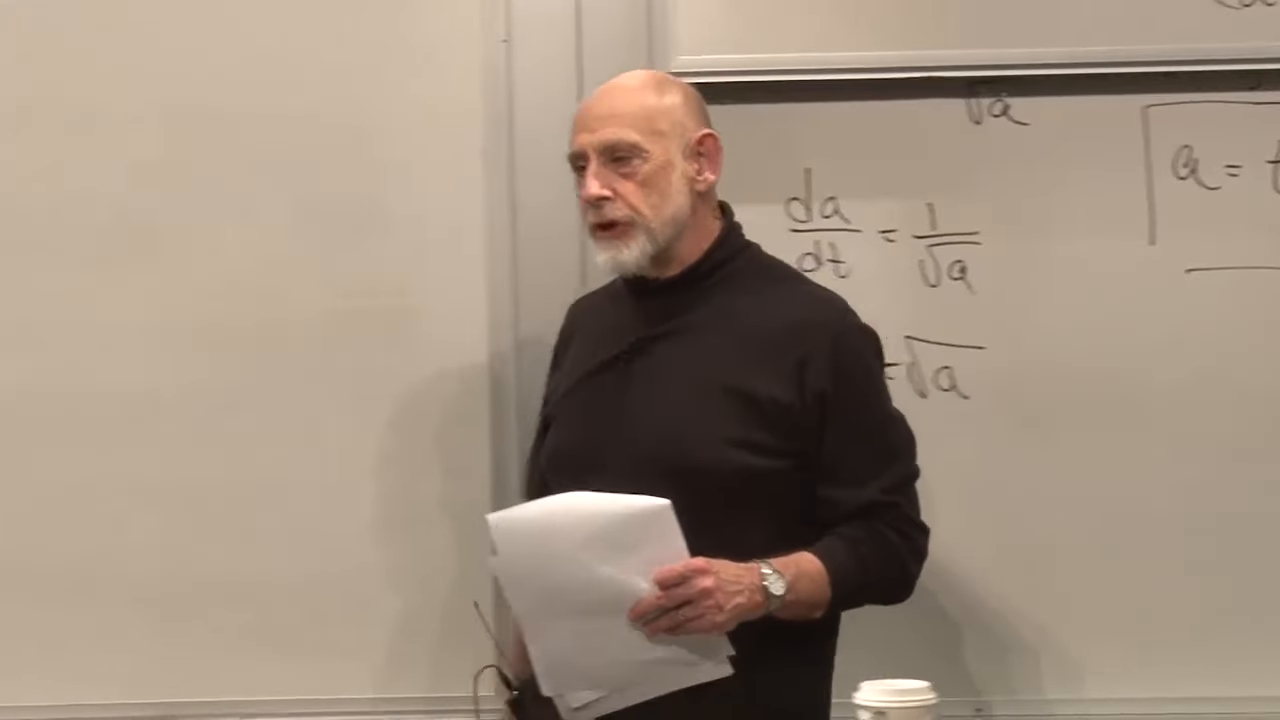
\includegraphics[width=0.68\textwidth]{lecture_02_figure_02.png}
\caption{Bảng tổng kết ghi \(\dot a=1/\sqrt a\) và định luật bị chi phối bởi vật chất, được đóng khung, \(a\propto t^{2/3}\). Phần đại số trung gian bị che khuất một phần và được bổ sung bởi các phương trình~\eqref{eq:c02-zero-energy-friedmann}--\eqref{eq:c02-matter-law}.}
\label{fig:c02-matter-recap}
\lectureframe{00:29:20.838}
\end{figure}

\begin{classroomqa}
\audiencequestion{Vì sao căn bậc hai âm bị loại bỏ?}
\lecturerresponse{Phương trình không loại bỏ nó. Phương trình~\eqref{eq:c02-zero-energy-friedmann} xác định \(H^2\), chứ không xác định dấu của \(H\). Nghiệm dương mô tả sự giãn nở và nghiệm âm mô tả sự co lại. Một hòn đá trong trường hấp dẫn của một hành tinh có thể đang chuyển động ra ngoài hoặc vào trong mà vẫn tuân theo cùng một phương trình năng lượng; điều kiện đầu của nó chọn nhánh. Ta đã chọn nhánh giãn nở vì đó là vũ trụ đang được bàn tới. \lecturetimestamp{00:23:09--00:24:46}}
\end{classroomqa}

Mô hình tiếp theo vẫn sẽ bỏ qua năng lượng tối. Sự bỏ qua đó là có chủ ý: trước hết ta hiểu khuôn khổ cũ gồm vật chất và bức xạ rồi mới thêm thành phần chi phối kỷ nguyên gia tốc hiện nay. Ngược lại, vật chất tối đã được gộp vào hạng vật chất vì vật chất tối phi tương đối tính cũng suy giảm theo \(a^{-3}\).

\begin{classroomqa}
\audiencequestion{Chẳng phải ngày nay năng lượng tối là thành phần trội sao?}
\lecturerresponse{Đúng. Câu chuyện hai thành phần được trình bày ở đây là vũ trụ học sư phạm chuẩn từ trước khi khám phá ra gia tốc hiện nay. Vật chất tối thuộc về nhóm vật chất; năng lượng tối là thành phần thứ ba sẽ được đưa vào riêng. Bắt đầu từ mô hình cũ giúp ta thấy mỗi hạng bổ sung làm thay đổi điều gì. \lecturetimestamp{00:28:02--00:28:45}}
\end{classroomqa}

\section{Khôi phục hằng số năng lượng}

Lựa chọn năng lượng bằng 0 là một điều kiện đầu đặc biệt. Để bỏ nó đi, hãy trở lại với một thiên hà khối lượng \(m\) ở biên của một hình cầu đồng nhất. Gọi bán kính đồng chuyển động của nó là \(x\), sao cho
\begin{equation}
D=ax,
\qquad
\dot D=\dot a x.
\label{eq:c02-comoving-particle}
\end{equation}
Định lý vỏ cầu của Newton nói rằng chỉ khối lượng \(M(D)\) ở bên trong hình cầu mới ảnh hưởng đến gia tốc xuyên tâm; các vỏ cầu ở bên ngoài không tác dụng lực tổng cộng nào. Năng lượng Newton bảo toàn của thiên hà là
\begin{equation}
\frac{1}{2}m\dot D^{\,2}-\frac{GM(D)m}{D}=E.
\label{eq:c02-newton-energy}
\end{equation}
Thừa số \(m\) phải có trong cả hai hạng. Khi viết nhanh trên bảng rất dễ bỏ sót nó, nhưng giữ lại nó làm rõ rằng hằng số cuối cùng là năng lượng trên một đơn vị khối lượng thử.

Tính đồng nhất cho phép ta chọn thiên hà đại diện tại \(x=1\). Khi đó \(D=a\), \(\dot D=\dot a\), và hình cầu có
\begin{equation}
V_{\rm sph}=\frac{4\pi}{3}a^3,
\qquad
M(a)=\rho_m V_{\rm sph}=\frac{4\pi}{3}\rho_m a^3.
\label{eq:c02-enclosed-mass}
\end{equation}
Trên bảng, \(V\) được dùng cả cho thể tích lẫn, trong một chú thích bên lề, cho vận tốc xuyên tâm. Ta sẽ giữ các ký hiệu rõ nghĩa \(V_{\rm sph}\) và \(\dot D\).

\begin{figure}[ht]
\centering
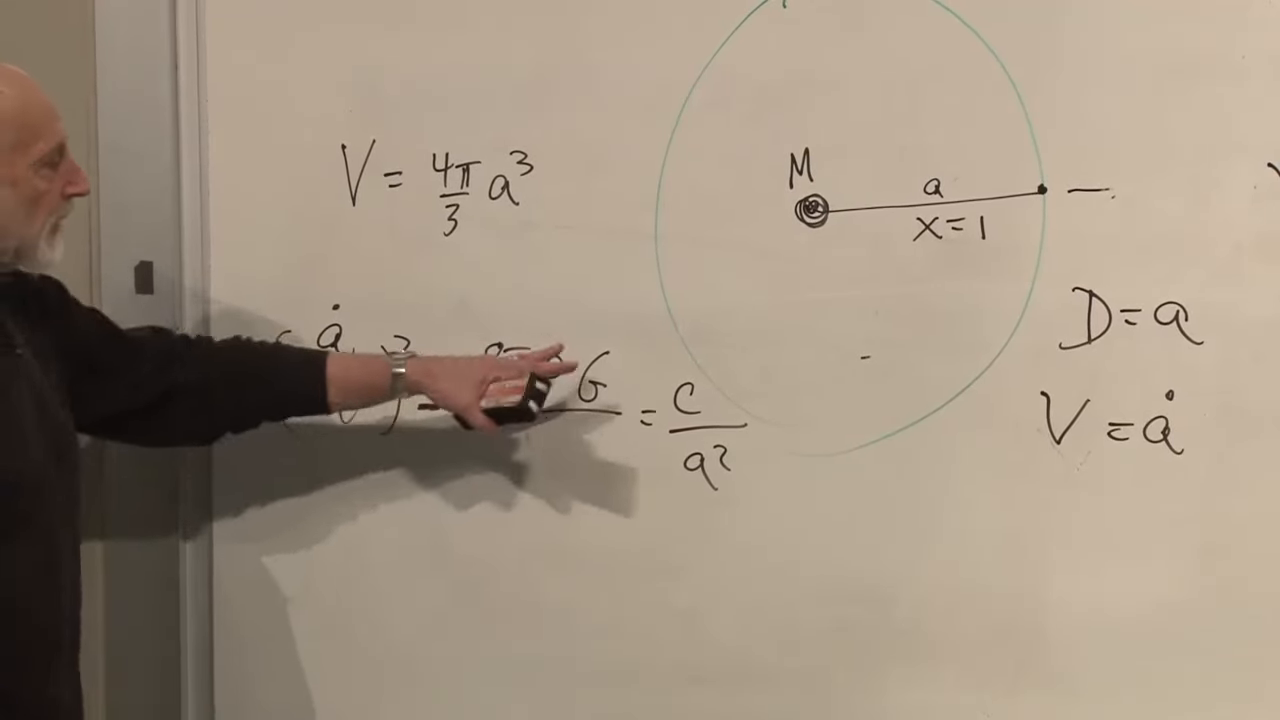
\includegraphics[width=0.86\textwidth]{lecture_02_figure_03.png}
\caption{Hình cầu khối lượng bao trong và phương trình Friedmann với năng lượng khác không. Các nhãn nhìn thấy được gồm \(V_{\rm sph}=4\pi a^3/3\), khối lượng ở tâm \(M\), \(x=1\), \(D=a\) và \(\dot D=\dot a\). Một phần của phương trình bị giảng viên che khuất và được khôi phục bằng đại số ở bên dưới.}
\label{fig:c02-energy-board}
\lectureframe{00:37:59.876}
\end{figure}

\begin{figure}[ht]
\centering
\begin{tikzpicture}[scale=1.05,>=Latex]
  \draw[thick] (0,0) circle (2.6);
  \fill (0,0) circle (2.2pt) node[below left=2pt] {\(M(a)\)};
  \draw[thick,->] (0,0) -- (2.58,0);
  \fill (2.6,0) circle (2.2pt) node[right=4pt] {galaxy \(m\)};
  \node[above] at (1.30,0.04) {\(D=ax\)};
  \node[below] at (1.30,-0.04) {\(x=1\Rightarrow D=a\)};
  \draw[->,blue!60!black,thick] (2.63,0.18) -- (3.55,0.72)
    node[right] {\(\dot D=\dot a\)};
  \node at (0,-3.05) {\(M(a)=\frac{4\pi}{3}\rho_m a^3\)};
\end{tikzpicture}
\caption{Bản dựng lại rõ ràng của hình cầu Newton tại \(x=1\). Các vỏ ở bên ngoài triệt tiêu nhau, nên thiên hà ở biên chỉ chịu tác dụng của khối lượng bao chứa.}
\label{fig:c02-sphere-redraw}
\end{figure}

Thay \(D=a\) vào phương trình~\eqref{eq:c02-newton-energy}, chia cho \(m/2\), và định nghĩa hằng số
\begin{equation}
C\equiv\frac{2E}{m}.
\end{equation}
Ta thu được
\begin{equation}
\dot a^{\,2}-\frac{2GM(a)}{a}=C.
\label{eq:c02-energy-a}
\end{equation}
Chia cho \(a^2\) và dùng phương trình~\eqref{eq:c02-enclosed-mass} cho
\begin{equation}
\left(\frac{\dot a}{a}\right)^2-
\frac{8\pi G}{3}\rho_m=\frac{C}{a^2},
\label{eq:c02-energy-form}
\end{equation}
hay tương đương,
\begin{equation}
\boxed{H^2=\frac{8\pi G}{3}\rho_m+\frac{C}{a^2}.}
\label{eq:c02-friedmann-C}
\end{equation}
Đây là phương trình Friedmann thứ nhất cho vật chất không áp suất, được viết theo quy ước năng lượng Newton. Hạng mới \(a^{-2}\) ghi nhớ việc thiên hà đại diện đã được phóng ra với năng lượng lớn hơn, bằng hay nhỏ hơn năng lượng thoát.

Thay \(\rho_m=\nu_m/a^3\) vào, thuận tiện là định nghĩa
\begin{equation}
A_m\equiv\frac{8\pi G\nu_m}{3}>0,
\end{equation}
để rồi
\begin{equation}
H^2=\frac{A_m}{a^3}+\frac{C}{a^2},
\qquad
\dot a^{\,2}=\frac{A_m}{a}+C.
\label{eq:c02-energy-branches}
\end{equation}
Phương trình này cho nhiều thông tin hơn khi xét các giới hạn hơn là đem tích phân ngay lập tức.

\subsection{Năng lượng dương}

Nếu \(C>0\), hạng vật chất \(A_m/a^3\) chi phối khi \(a\) nhỏ. Vì vậy, sự giãn nở ở giai đoạn sớm vẫn giữ quy luật vật chất \(a\propto t^{2/3}\). Tuy nhiên, khi \(a\) lớn, hạng \(C/a^2\) lại chi phối trong \(H^2\), hay tương đương là
\begin{equation}
\dot a^{\,2}\longrightarrow C.
\end{equation}
Sự giãn nở tiến gần tới tốc độ không đổi,
\begin{equation}
a(t)\sim\sqrt C\,t.
\label{eq:c02-positive-late}
\end{equation}
Đây là đối ứng vũ trụ học của việc ném một quả táo với tốc độ lớn hơn vận tốc thoát. Trọng lực liên tục làm giảm tốc độ của nó, nhưng ở rất xa, quả táo vẫn giữ một vận tốc tiệm cận khác không.

\subsection{Năng lượng bằng 0}

Với \(C=0\), phương trình~\eqref{eq:c02-energy-branches} cho nghiệm tới hạn \(a\propto t^{2/3}\). Nó giãn nở vô hạn trong khi \(\dot a\) tiến về 0. Đây chính là trường hợp đúng bằng năng lượng thoát.

\subsection{Năng lượng âm}

Nếu \(C=-|C|<0\), thì
\begin{equation}
H^2=\frac{A_m}{a^3}-\frac{|C|}{a^2}
=\frac{A_m-|C|a}{a^3}.
\label{eq:c02-negative-energy}
\end{equation}
thừa số tỉ lệ không thể vượt quá
\begin{equation}
a_{\max}=\frac{A_m}{|C|},
\label{eq:c02-amax}
\end{equation}
vì vế phải đạt tới 0 tại đó. Nhánh giãn nở đi tới \(a_{\max}\) với \(\dot a=0\); phần tiếp nối là nhánh co lại. Trong bức tranh Newton, đây là một quả táo được phóng với vận tốc nhỏ hơn vận tốc thoát: nó bay lên, quay đầu, rồi rơi xuống.

\begin{classroomqa}
\audiencequestion{Làm sao mô hình có thể tái co sụp khi vế phải bằng \(H^2\) và do đó không thể âm?}
\lecturerresponse{Nó không bao giờ trở thành âm. Trong quá trình giãn nở, vế phải giảm về 0 tại \(a_{\max}\). Ở đó \(H=0\). Khi ấy nghiệm chuyển từ căn bậc hai dương sang căn bậc hai âm và lần ngược lại miền được phép với \(\dot a<0\). Một cách tiếp diễn có vẻ hấp dẫn nhưng sai sẽ để cho biểu thức đi xuyên qua 0. Điều đó không thể xảy ra: 0 là biên, không phải là một giá trị mà qua đó một \(H\) thực có thể tiếp tục. \lecturetimestamp{00:48:43--00:53:03}}
\end{classroomqa}

Vì vậy, ba giá trị năng lượng Newton cho ba lịch sử định tính: tái co sụp với \(C<0\), thoát tới hạn với \(C=0\), và giãn nở vĩnh viễn với \(\dot a\) tiệm cận một hằng số đối với \(C>0\). Bước tiếp theo đầy bất ngờ là thuyết tương đối rộng gán cho chính các trường hợp này một ý nghĩa hình học.

\section{Từ năng lượng đến độ cong}

Chuyển hạng năng lượng trong phương trình~\eqref{eq:c02-friedmann-C} sang vế hình học và định nghĩa
\begin{equation}
k\equiv-C.
\label{eq:c02-k-definition}
\end{equation}
Khi đó
\begin{equation}
\boxed{H^2+\frac{k}{a^2}=\frac{8\pi G}{3}\rho.}
\label{eq:c02-friedmann-k}
\end{equation}
Trên bảng, ký hiệu luân phiên giữa \(C\), \(K\) và \(\kappa\), và một dấu được hấp thụ khi chuyển hạng ấy qua dấu bằng. Phương trình~\eqref{eq:c02-k-definition} cố định quy ước của ta: năng lượng Newton dương tương ứng với \(k<0\), năng lượng bằng 0 tương ứng với \(k=0\), và năng lượng Newton âm tương ứng với \(k>0\).

\begin{figure}[ht]
\centering
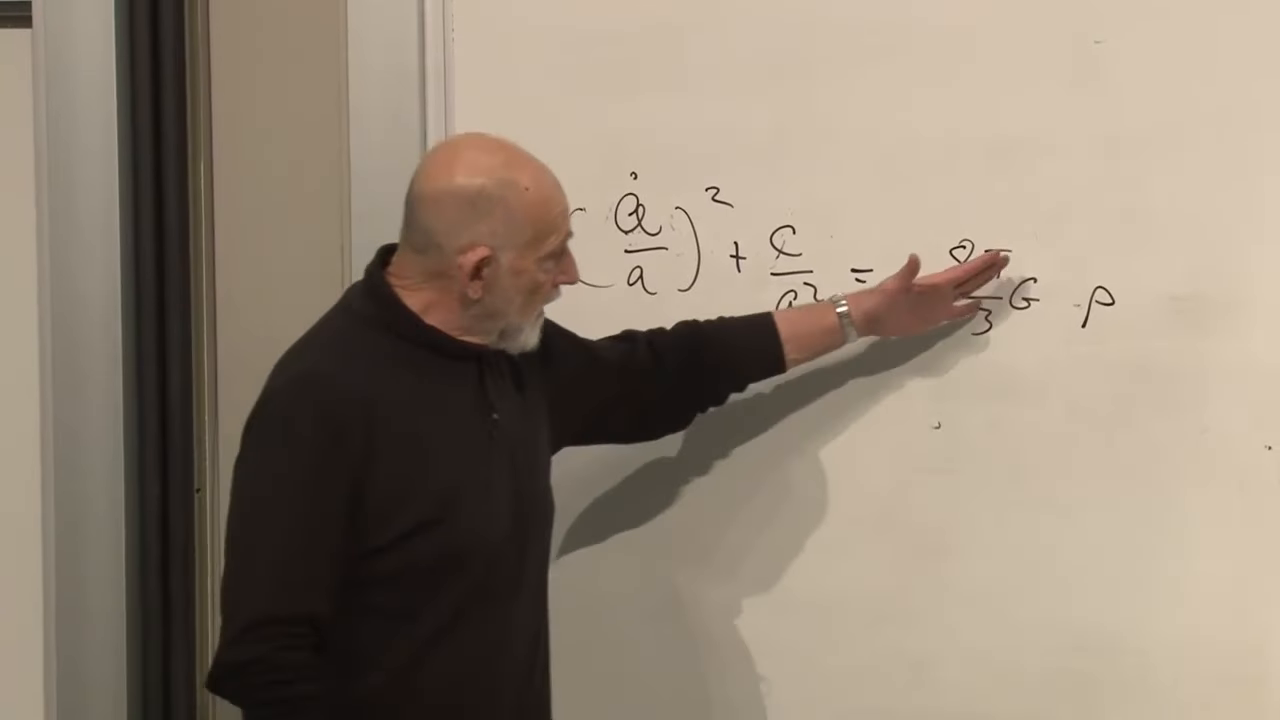
\includegraphics[width=0.76\textwidth]{lecture_02_figure_04.png}
\caption{Phương trình Friedmann được sắp xếp với hình học ở vế trái và nguồn ở vế phải. Khung hình hỗ trợ sự phân chia khái niệm này; nó không hiển thị đầy đủ phương trình tensor Einstein.}
\label{fig:c02-geometry-source}
\lectureframe{00:55:22.810}
\end{figure}

Cách sắp xếp này là một phiên bản thu nhỏ của phương trình Einstein. Vế trái mô tả hình học: sự giãn nở qua \(H\), và độ cong không gian qua \(k/a^2\). Vế phải mô tả nguồn vật chất. Trong cơ học Newton, nguồn đó là mật độ khối lượng. Trong thuyết tương đối, đó là năng lượng và xung lượng, được biểu diễn đầy đủ bởi tensor năng lượng-động lượng. Đối với một vũ trụ đồng nhất và đẳng hướng, phương trình Friedmann thứ nhất phụ thuộc vào tổng mật độ năng lượng \(\rho\).

Nếu giữ các đơn vị thông thường, một mật độ khối lượng đóng góp thông qua năng lượng nghỉ của nó \(\rho_{\rm mass}c^2\). Từ đây trở đi, ta đặt \(c=1\), nên khối lượng và năng lượng dùng cùng đơn vị. Khi đó ký hiệu \(\rho\) có thể bao gồm khối lượng nghỉ, động năng, bức xạ, và bất kỳ thành phần năng lượng đồng nhất nào khác.

\begin{figure}[ht]
\centering
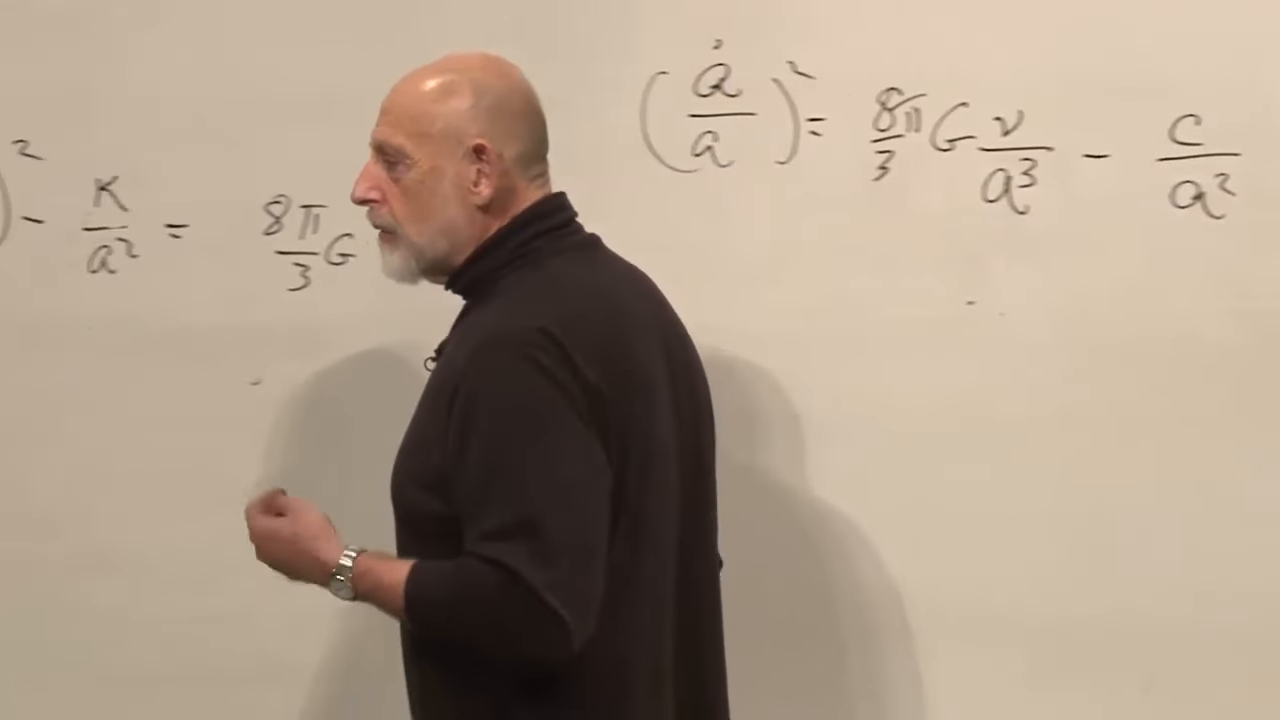
\includegraphics[width=0.88\textwidth]{lecture_02_figure_05.png}
\caption{Các dạng trên bảng đặt cạnh nhau của phương trình Friedmann: một dạng độ cong dùng \(\rho\), và một dạng vật chất thu được sau khi \(\rho_m=\nu_m/a^3\). Ký hiệu trên bảng có thay đổi; phương trình~\eqref{eq:c02-k-definition} giữ quy ước dấu cố định ở đây.}
\label{fig:c02-curvature-comparison}
\lectureframe{00:57:52.659}
\end{figure}

Cách diễn giải hình học này mang tính toàn cục. Trong mô hình tương đối tính, \(k=0\) mô tả các lát không gian phẳng, \(k>0\) các lát hình cầu có độ cong dương, và \(k<0\) các lát hyperbol có độ cong âm. Phép suy dẫn Newton tái tạo cùng một phương trình tiến hóa mà không có những hình học toàn cục này. Vì vậy, hằng số năng lượng khác không của nó mô phỏng độ cong một cách chính xác đáng kinh ngạc, nhưng không tự nó suy dẫn ra chính không gian cong.

\begin{classroomqa}
\audiencequestion{Làm sao cơ học Newton và thuyết tương đối rộng có thể cho cùng một phương trình giãn nở nếu hình học của chúng khác nhau?}
\lecturerresponse{Thuyết tương đối rộng bao gồm trường hợp phẳng, và cục bộ thì mọi hình học trơn đều xấp xỉ phẳng. Đáng chú ý hơn, hằng số năng lượng Newton đi vào phương trình tiến hóa đúng ngay vị trí mà độ cong không gian tương đối tính chiếm giữ. Công thức động lực học thì trùng khớp, còn cách diễn giải toàn cục thì không: không gian Newton Euclid không hề âm thầm trở thành một không gian cầu hay một không gian siêu bôlic. Ba hình học đó sẽ phải được xây dựng trong khuôn khổ thuyết tương đối rộng. \lecturetimestamp{01:20:59--01:24:20}}
\end{classroomqa}

\section{Bức xạ trong một hộp giãn nở}

Bây giờ ta thay đổi thành phần của vũ trụ. Hãy xét một khối lập phương đơn vị đồng chuyển động. Thể tích vật lý của nó là \(a^3\). Đối với vật chất phi tương đối tính, số hạt trong hộp đó là cố định và năng lượng nghỉ của mỗi hạt xấp xỉ cố định, nên có \(\rho_m\propto a^{-3}\). Đối với bức xạ còn có một hiệu ứng khác: mỗi photon mất năng lượng khi vũ trụ giãn nở.

Một photon có bước sóng \(\lambda\) có năng lượng
\begin{equation}
E_\gamma=\frac{hc}{\lambda},
\qquad
E_\gamma\propto\lambda^{-1}.
\label{eq:c02-photon-energy}
\end{equation}
Trong giãn nở đồng nhất, một bước sóng truyền tự do bị kéo giãn theo thừa số tỉ lệ:
\begin{equation}
\frac{\lambda(t_2)}{\lambda(t_1)}
=\frac{a(t_2)}{a(t_1)},
\qquad
\lambda\propto a.
\label{eq:c02-redshift}
\end{equation}
Đây là sự dịch đỏ vũ trụ học. Hệ quả là
\begin{equation}
E_\gamma\propto a^{-1}.
\label{eq:c02-photon-redshift}
\end{equation}
Nếu số photon trong hộp đồng chuyển động được bảo toàn, thì tổng năng lượng bức xạ của nó giảm theo \(a^{-1}\). Chia cho thể tích vật lý của nó \(a^3\) ta được
\begin{equation}
\boxed{\rho_r(a)=\frac{\nu_r}{a^4}.}
\label{eq:c02-radiation-density}
\end{equation}
Ở đây \(\nu_r\) là hệ số biên độ không đổi của mật độ bức xạ truyền tự do. Bức xạ có thêm một lũy thừa nghịch đảo của \(a\) so với vật chất: ba lũy thừa do sự pha loãng không gian và một lũy thừa do sự dịch đỏ của mỗi photon.

Phép tương tự với dây đàn guitar cho trực giác hữu ích. Một mode khớp với một sợi dây có một số nguyên nửa bước sóng. Nếu sợi dây được kéo dài chậm, số nguyên đó không thể thay đổi liên tục; thay vào đó, bước sóng điều chỉnh theo độ dài mới. Tương tự, đối với một sóng trên một vòng đang nở chậm, số nút là một bất biến đoạn nhiệt, nên bước sóng của nó bám theo chu vi. Một sóng tổng quát có thể được phân tích thành các mode như vậy.

Đây không phải là sự thay thế cho việc giải các phương trình Maxwell trong một không-thời gian đang giãn nở. Nó là trực giác được kiểm soát đứng sau phương trình~\eqref{eq:c02-redshift}: sự giãn nở hình học chậm làm thay đổi bước sóng vật lý trong khi vẫn giữ nguyên nhãn mode.

\begin{classroomqa}
\audiencequestion{Lập luận này có đòi hỏi một hộp dẫn điện hoặc phản xạ không? Điều gì xảy ra trong không gian rỗng đang giãn nở mà không có các vách vật lý?}
\lecturerresponse{Các vách chỉ là một công cụ hạch toán, chứ không phải khẳng định rằng vũ trụ được bao kín bởi một vật dẫn. Một chứng minh đầy đủ xuất phát từ sự truyền sóng trong metric đang giãn nở. Đối với lập luận hiện tại, ta dùng sự kiện đã được quan sát và được suy ra bằng thuyết tương đối rằng các bước sóng truyền tự do tỉ lệ theo \(a\). Chiếc hộp giúp đếm photon và thể tích vật lý; nó không gây ra sự dịch đỏ vũ trụ học. \lecturetimestamp{01:02:21--01:04:37}}
\end{classroomqa}

\begin{classroomqa}
\audiencequestion{Vì sao một bước sóng phải bám theo lưới thay vì giữ một độ dài vật lý cố định?}
\lecturerresponse{Hãy xét một mode trên một vòng có chu vi biến đổi đoạn nhiệt. Số nút của nó là một số nguyên nên không thể trôi liên tục, vì vậy bước sóng được phép phải biến đổi theo vòng. Khai triển một sóng tổng quát thành các mode Fourier cho cùng kết luận trên từng mode. Điều này cung cấp trực giác đoạn nhiệt cần thiết; phát biểu chính xác thuộc về lý thuyết trường trong không-thời gian cong. \lecturetimestamp{01:34:18--01:38:33}}
\end{classroomqa}

\subsection{Nghiệm chi phối bởi bức xạ}

Tạm thời bỏ qua độ cong, thế phương trình~\eqref{eq:c02-radiation-density} vào phương trình Friedmann:
\begin{equation}
H^2=\frac{8\pi G\nu_r}{3a^4}
\equiv\frac{A_r}{a^4},
\qquad A_r>0.
\label{eq:c02-radiation-friedmann}
\end{equation}
Trên nhánh giãn nở,
\begin{equation}
\frac{\dot a}{a}=\frac{\sqrt{A_r}}{a^2},
\qquad
\dot a=\frac{\sqrt{A_r}}{a}.
\end{equation}
Do đó
\begin{equation}
a\,da=\sqrt{A_r}\,dt,
\qquad
\frac{a^2}{2}=\sqrt{A_r}(t-t_B),
\end{equation}
và
\begin{equation}
\boxed{a(t)\propto(t-t_B)^{1/2}.}
\label{eq:c02-radiation-law}
\end{equation}
Sự khác biệt giữa các số mũ \(1/2\) và \(2/3\) nhìn thì nhỏ nhưng quyết định về mặt vật lý. Tốc độ giãn nở, nhiệt độ, sự đóng băng phản ứng, và kích thước chân trời trong vũ trụ sơ khai đều phụ thuộc vào thành phần nào chi phối.

\section{Vũ trụ gồm vật chất và bức xạ}

Đối với vật chất và bức xạ được bảo toàn riêng rẽ, các mật độ của chúng cộng lại:
\begin{equation}
\rho(a)=\rho_m(a)+\rho_r(a).
\end{equation}
Bỏ qua độ cong trong phép so sánh này,
\begin{equation}
\boxed{H^2=\frac{C_m}{a^3}+\frac{C_r}{a^4},}
\label{eq:c02-mixed-friedmann}
\end{equation}
trong đó \(C_m,C_r>0\). Trên bảng trước tiên hai hệ số được ký hiệu là \(C_1\) và \(C\); ký hiệu thứ hai sau đó được sửa bằng lời thành một hằng số riêng biệt. Ký hiệu trong phương trình~\eqref{eq:c02-mixed-friedmann} làm cho sự sửa đó trở nên tường minh.

\begin{figure}[ht]
\centering
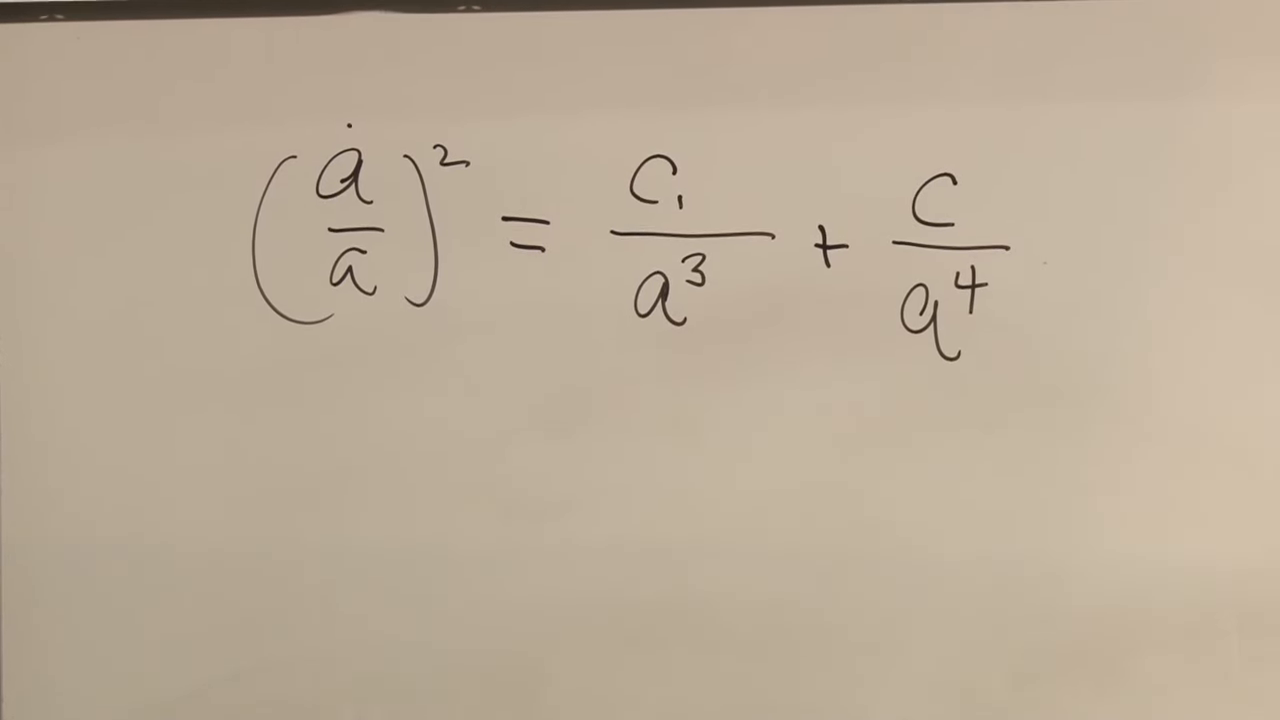
\includegraphics[width=0.74\textwidth]{lecture_02_figure_06.png}
\caption{Phương trình hỗn hợp vật chất–bức xạ trên bảng. Hệ số thứ hai được viết trên bảng sau đó được sửa thành một hằng số riêng cho bức xạ, ký hiệu là \(C_r\) trong phương trình~\eqref{eq:c02-mixed-friedmann}.}
\label{fig:c02-mixed-board}
\lectureframe{01:11:37.997}
\end{figure}

Ở \(a\) nhỏ, hạng bức xạ trội hơn vì \(a^{-4}\) tăng nhanh hơn \(a^{-3}\):
\begin{equation}
a\ll a_{\rm eq}
\quad\Longrightarrow\quad
H^2\simeq\frac{C_r}{a^4},
\qquad
a(t)\propto t^{1/2}.
\end{equation}
Ở \(a\) lớn hơn, vật chất trội hơn:
\begin{equation}
a\gg a_{\rm eq}
\quad\Longrightarrow\quad
H^2\simeq\frac{C_m}{a^3},
\qquad
a(t)\propto t^{2/3}.
\end{equation}
Thang cân bằng suy ra trực tiếp bằng cách cho hai hạng bằng nhau:
\begin{equation}
a_{\rm eq}=\frac{C_r}{C_m}.
\label{eq:c02-equality-scale}
\end{equation}
Sự cân bằng này không phải là cùng một sự kiện với sự tách ghép photon. Cân bằng hỏi khi nào hai mật độ năng lượng bằng nhau; tách ghép hỏi khi nào các tương tác không còn giữ cho vật chất và bức xạ ở tiếp xúc nhiệt.

Thành phần bức xạ bao gồm photon và mọi loại hạt chuyển động siêu tương đối tính. Các neutrino rất nhẹ ứng xử như vậy ở nhiệt độ đủ cao, và một phông graviton cũng sẽ biến thiên theo cùng cách đó. Khi một loại hạt có khối lượng trở nên phi tương đối tính, đóng góp khối lượng nghỉ chi phối của nó bắt đầu biến thiên như vật chất. Vật chất tối lạnh thuộc \(C_m/a^3\), không thuộc hạng bức xạ.

\begin{classroomqa}
\classquestion{Hạng nào trong phương trình~\eqref{eq:c02-mixed-friedmann} chi phối trước, và hạng nào chi phối về sau?}
\lecturerresponse{Đối với \(a\) nhỏ, \(a^{-4}\) trội hơn \(a^{-3}\), nên bức xạ chi phối sự giãn nở sớm và cho \(a\propto t^{1/2}\). Khi \(a\) tăng, tỷ số bức xạ trên vật chất giảm như \(1/a\); khi đó vật chất chi phối sự giãn nở và cho \(a\propto t^{2/3}\). \lecturetimestamp{01:11:46--01:13:38}}
\end{classroomqa}

\begin{classroomqa}
\audiencequestion{Có đang giả sử rằng lượng tương đối của vật chất và bức xạ là không đổi không?}
\lecturerresponse{Mật độ của chúng không hằng, nhưng các hệ số \(C_m\) và \(C_r\) có thể được coi là hằng sau khi các thành phần ngừng trao đổi năng lượng một cách hiệu quả và việc tạo ra hay hủy diệt hạt là không đáng kể. Khi đó, vật chất mang một khối lượng nghỉ đồng hành được bảo toàn, còn bức xạ tự do mang một số photon đồng hành được bảo toàn, với dịch đỏ cung cấp cho nó thừa số bổ sung \(a^{-1}\). Trong những thời kỳ tương tác mạnh hoặc hủy diệt các loại hạt, cách hạch toán này phải được tinh chỉnh. \lecturetimestamp{01:13:39--01:14:53}}
\end{classroomqa}

\begin{classroomqa}
\audiencequestion{Khi nào vật chất và bức xạ ngừng tương tác mạnh với nhau?}
\lecturerresponse{Một câu trả lời gần đúng theo bậc độ lớn là \(10^5\) năm cho thời điểm photon tách rời khỏi vật chất thông thường. Lịch sử tái hợp chính xác là một phép tính về sau, và không nên nhầm nó với thời điểm bằng nhau vật chất--bức xạ. Điều cần ở đây chỉ là, sau khi tách rời, hai thành phần có thể được theo dõi xấp xỉ một cách riêng rẽ. \lecturetimestamp{01:27:29--01:27:46}}
\end{classroomqa}

\begin{classroomqa}
\audiencequestion{Làm sao chúng ta có thể biết rằng đã có một kỷ nguyên sớm \(a\propto t^{1/2}\) trước khi tồn tại các thiên hà để lần theo sự giãn nở?}
\lecturerresponse{Chúng ta suy ra lịch sử giãn nở từ những ghi chép vật lý mà nó để lại. Tổng hợp hạt nhân nguyên thủy phụ thuộc vào sự cạnh tranh sớm giữa các tốc độ phản ứng và \(H(t)\); phông vi sóng ghi lại trạng thái nhiệt và các nhiễu loạn ở giai đoạn muộn hơn. Các quan sát thiên hà làm cho hành vi của thời kỳ vật chất trở nên trực tiếp hơn, còn thời kỳ bức xạ được tái dựng từ bằng chứng này của vũ trụ sơ khai. \lecturetimestamp{01:27:46--01:30:10}}
\end{classroomqa}

Mô hình vật chất cộng bức xạ được cố ý giữ ở dạng chưa hoàn chỉnh. Đó là khuôn khổ kinh điển trong đó vũ trụ chuyển từ thời kỳ bức xạ chi phối sang thời kỳ vật chất chi phối. Sự giãn nở tăng tốc hiện nay đòi hỏi một nguồn khác là năng lượng tối, nguồn này sẽ thêm vào một hạng khác biệt về mặt định tính.

\section{Năng lượng do dịch đỏ đi đâu}

Sự suy giảm \(E_\gamma\propto a^{-1}\) đặt ra một câu hỏi không thể tránh khỏi: năng lượng photon đã đi đâu? Trong một cái hộp thực sự đang giãn nở với các thành phản xạ, bức xạ tác dụng áp suất và thực hiện công lên các thành. Phát biểu nhiệt động lực học là
\begin{equation}
dE=-p\,dV.
\label{eq:c02-pdv}
\end{equation}
Khi \(V\) tăng, năng lượng bức xạ giảm. Phần năng lượng mất đi có thể xuất hiện dưới dạng động năng, biến dạng hoặc nhiệt trong bất cứ thứ gì làm cho các thành chuyển động.

Hộp đồng hành không có các thành vật chất. Nó là một biên tưởng tượng chuyển động cùng sự giãn nở trung bình. Các photon đi qua nó, nhưng trong một bể bức xạ đồng nhất, thông lượng thống kê đi vào cân bằng với thông lượng đi ra. Hộp ấy vẫn là một thể tích hạch toán hợp lệ dù không phải là một vật chứa. Định luật công do áp suất vẫn mô tả cách năng lượng trong một thể tích đồng hành tiến hóa.

Đối với bức xạ, \(p=\rho/3\), và \(E=\rho V\). Khi đó phương trình~\eqref{eq:c02-pdv} cho
\begin{align}
d(\rho V)&=-\frac{\rho}{3}\,dV,\\
V\,d\rho&=-\frac{4}{3}\rho\,dV,\\
\frac{d\rho}{\rho}&=-\frac{4}{3}\frac{dV}{V}.
\end{align}
Vì \(V\propto a^3\), lấy tích phân cho \(\rho\propto a^{-4}\), phù hợp với lập luận dựa trên bước sóng. Cách suy dẫn nhiệt động lực học này cũng cho thấy rõ rằng không chỉ mật độ số giảm đi, mà năng lượng của từng photon cũng giảm.

\begin{classroomqa}
\audiencequestion{Năng lượng của các photon bị dịch đỏ đi đâu? Tổng năng lượng của vũ trụ có được bảo toàn không?}
\lecturerresponse{Với các thành vật lý, bức xạ thực hiện công lên chúng, nên sự chuyển giao là hạch toán cơ học thông thường. Đối với toàn bộ vũ trụ, câu hỏi này tinh tế hơn. Bảo toàn năng lượng toàn cục thông thường là hệ quả của đối xứng tịnh tiến theo thời gian, nhưng một không-thời gian giãn nở nói chung không bất biến dưới phép tịnh tiến theo thời gian và không nhất thiết phải có một tổng năng lượng bảo toàn duy nhất. Người ta có thể xây dựng những phép tương tự Newton hữu ích liên quan đến năng lượng của sự giãn nở, nhưng một phát biểu toàn cục dứt khoát đòi hỏi thuyết tương đối rộng. Cả hai cách mô tả đều hữu ích ở đây, nhưng từ mô hình Newton không suy ra được một kết luận toàn cục chung cuộc. \lecturetimestamp{01:16:51--01:20:58}}
\end{classroomqa}

\begin{classroomqa}
\audiencequestion{Nếu hộp đồng hành là tưởng tượng và photon đi qua biên của nó, thì cách hình dung bằng công do áp suất vẫn hữu ích như thế nào?}
\lecturerresponse{Tính đồng nhất cung cấp phần hạch toán còn thiếu. Trung bình, mỗi photon rời khỏi một thể tích đồng hành sẽ được thay thế về mặt thống kê bằng một photon đi vào từ vùng lân cận. Các thông lượng cục bộ triệt tiêu nhau về trung bình, trong khi thể tích vật lý và bước sóng thay đổi. Một hộp phản xạ làm cho cơ chế công trở nên cụ thể; hộp đồng hành mang cùng định luật bảo toàn trung bình đó mà không cần các thành theo nghĩa đen. \lecturetimestamp{01:24:22--01:27:28}}
\end{classroomqa}

\begin{classroomqa}
\audiencequestion{Sự giãn nở chỉ làm giảm mật độ photon, hay còn làm giảm năng lượng của từng photon?}
\lecturerresponse{Cả hai đều xảy ra. Số photon trên mỗi thể tích vật lý giảm như \(a^{-3}\), và dịch đỏ vũ trụ học làm giảm năng lượng của mỗi photon thêm một thừa số \(a^{-1}\). Đây là phép tương tự trong bức xạ của sự làm lạnh đoạn nhiệt. Một chất khí thông thường cũng lạnh đi khi thực hiện công trong quá trình giãn nở chậm, mặc dù giãn nở tự do đột ngột là một quá trình nhiệt động lực học khác. \lecturetimestamp{01:42:30--01:45:55}}
\end{classroomqa}

\section{Sự lùi xa, các chân trời và giới hạn của mô hình}

Định luật Hubble gán tốc độ lùi xa
\begin{equation}
v_{\rm rec}=HD
\label{eq:c02-recession}
\end{equation}
cho một vật thể ở khoảng cách riêng \(D\) trên một lát cắt thời gian vũ trụ được chọn. Với \(D\) đủ lớn, phương trình~\eqref{eq:c02-recession} có thể vượt quá \(c\). Điều này không vi phạm thuyết tương đối hẹp, vì \(v_{\rm rec}\) không phải là vận tốc của một vật thể lân cận được đo trong một hệ quy chiếu quán tính địa phương duy nhất. Nó so sánh các đường thế đồng hành cách xa nhau trong một hình học đang biến đổi. Mọi quan sát viên địa phương vẫn đo ánh sáng với tốc độ \(c\), và không có vật thể vật chất địa phương nào vượt qua vật thể khác nhanh hơn ánh sáng.

\begin{classroomqa}
\audiencequestion{Một thiên hà ở đủ xa có thể lùi xa nhanh hơn ánh sáng không?}
\lecturerresponse{Có, tốc độ lùi xa vũ trụ học \(HD\) của nó có thể vượt quá \(c\). Khi đó không có vật thể địa phương nào vượt qua một quan sát viên lân cận nhanh hơn ánh sáng, và kết quả này không thể được dùng cho truyền tín hiệu siêu ánh sáng. Đây là một phát biểu về sự thay đổi khoảng cách riêng giữa các đường thế đồng hành ở xa, chứ không phải một vận tốc thông thường của thuyết tương đối hẹp được đo tại một biến cố. \lecturetimestamp{01:30:17--01:32:13}}
\end{classroomqa}

Bản thân sự lùi xa siêu ánh sáng không quyết định liệu ánh sáng phát ra bây giờ có bao giờ tới được chỗ ta hay không. Đó là một câu hỏi về toàn bộ lịch sử giãn nở trong tương lai. Trong một mô hình giảm tốc do vật chất chi phối, các vùng hiện đang lùi xa nhanh hơn ánh sáng về sau có thể trở nên quan sát được vì chân trời liên quan có tiến hóa. Nếu sự giãn nở tăng tốc còn tiếp diễn, một chân trời sự kiện có thể vĩnh viễn che khuất các biến cố ở đủ xa.

\begin{classroomqa}
\audiencequestion{Các thiên hà có biến mất một khi tốc độ lùi xa của chúng vượt quá tốc độ ánh sáng không?}
\lecturerresponse{Không đơn giản như vậy. Việc đi qua bán kính Hubble và một chân trời sự kiện thực sự là hai khái niệm khác nhau. Trong một mô hình giảm tốc, ánh sáng từ một vùng hiện đang lùi xa siêu ánh sáng vẫn có thể đến được chỗ ta về sau. Sự chi phối dai dẳng của năng lượng tối làm thay đổi cấu trúc nhân quả toàn cục và có thể tạo ra một chân trời tối hậu. Việc quyết định những tín hiệu nào đến nơi đòi hỏi hình học không-thời gian, chứ không phải một ảnh chụp tức thời của \(HD\). \lecturetimestamp{01:32:14--01:34:18}}
\end{classroomqa}

Ngôn ngữ của thuyết tương đối hẹp cũng có thể gây hiểu lầm khi áp dụng trên toàn cục. Khối lượng nghỉ bất biến của một hạt không tăng theo tốc độ. Năng lượng và động lượng của nó phụ thuộc vào hệ quy chiếu địa phương của quan sát viên. Các hạt có khối lượng không thể được gia tốc vượt qua tốc độ ánh sáng địa phương, nhưng sự lùi xa của một thiên hà đồng hành ở xa không phải là việc nó đi qua một hệ quy chiếu địa phương duy nhất.

\begin{classroomqa}
\audiencequestion{Một thiên hà lùi xa nhanh có thu được một khối lượng tương đối tính lớn hơn không?}
\lecturerresponse{Tốt hơn là không dùng ``khối lượng tương đối tính''. Thiên hà có một khối lượng nghỉ bất biến, còn năng lượng và động lượng của nó phụ thuộc vào hệ quy chiếu. Hơn nữa, một tốc độ lùi xa được gán trên khoảng cách vũ trụ học không phải là vận tốc địa phương xuất hiện trong công thức của thuyết tương đối hẹp. Các khái niệm này chỉ ăn khớp với nhau sau khi các biến cố ở xa được so sánh bằng metric không-thời gian. \lecturetimestamp{01:38:34--01:40:05}}
\end{classroomqa}

\begin{classroomqa}
\audiencequestion{Các trục thời gian và không gian sẽ ra sao khi tốc độ lùi xa ở khoảng cách lớn là siêu quang?}
\lecturerresponse{Không có một hệ quy chiếu Lorentz toàn cục duy nhất mà các trục nghiêng của nó có thể giải quyết được câu hỏi này. Thuyết tương đối hẹp so sánh các hệ quy chiếu quán tính trong không-thời gian phẳng; vũ trụ học đòi hỏi một mêtric liên hệ các hệ quy chiếu cục bộ trên một không-thời gian cong mở rộng. Lập luận Newton vẫn đáng tin cậy trong một miền nhỏ, nhưng cách xây dựng toàn cục phải đợi đến thuyết tương đối rộng. \lecturetimestamp{01:40:07--01:42:30}}
\end{classroomqa}

Bảo toàn năng lượng Newton đã cho ra phương trình hệ số tỉ lệ đúng cho vật chất và thậm chí còn báo trước hạng tử độ cong. Cơ học sóng và nhiệt động lực học cho quy luật tỉ lệ của bức xạ. Tuy nhiên, hình học không gian, năng lượng toàn cục và các chân trời không phải là những câu hỏi Newton cục bộ; chúng đòi hỏi mô tả mêtric tiếp theo.

\section{Vật chất, bức xạ và độ cong}

Nghiệm tới hạn chỉ gồm vật chất thỏa mãn
\begin{equation}
\rho_m\propto a^{-3},
\qquad
a(t)\propto t^{2/3}.
\end{equation}
Khi khôi phục năng lượng Newton trên mỗi đơn vị khối lượng, ta được
\begin{equation}
H^2=\frac{8\pi G}{3}\rho_m+\frac{C}{a^2}.
\end{equation}
\(C\) dương dẫn đến giãn nở vĩnh viễn với \(a\sim t\) ở thời muộn, \(C=0\) cho trường hợp thoát tới hạn, còn \(C\) âm cho một hệ số tỉ lệ cực đại rồi sau đó co sụp trở lại. Định nghĩa \(k=-C\) chuyển chính hạng tử đó sang vế hình học của phương trình Friedmann tương đối tính.

Bức xạ khác với vật chất vì sự giãn nở làm thay đổi cả mật độ số lẫn năng lượng trên mỗi lượng tử:
\begin{equation}
\begin{aligned}
\lambda&\propto a,
&\qquad E_\gamma&\propto a^{-1},\\
\rho_r&\propto a^{-4},
& a(t)&\propto t^{1/2}.
\end{aligned}
\end{equation}
Vì vậy, phương trình hai thành phần
\begin{equation}
H^2=\frac{C_m}{a^3}+\frac{C_r}{a^4}
\end{equation}
mô tả một vũ trụ sơ khai do bức xạ chi phối, tiếp theo là một kỷ nguyên do vật chất chi phối. Năng lượng tối, hình học không gian và cấu trúc nhân quả của các chân trời vẫn nằm ngoài mô hình này, đúng vào chỗ mà phép gần đúng Newton cho biết ta phải chuyển bài toán sang thuyết tương đối rộng.
